\documentclass[conference]{IEEEtran}
\IEEEoverridecommandlockouts

\usepackage{cite}
\usepackage{amsmath,amssymb,amsfonts}
\usepackage{graphicx}
\usepackage{textcomp}
\usepackage{xcolor}
\usepackage{booktabs}
\usepackage{url}
\usepackage{tikz}
\usetikzlibrary{positioning,arrows.meta,fit,backgrounds}
\graphicspath{{figures/}}

\begin{document}

\title{Explainable Music Genre and Mood Classification Using Audio Features}

\author{
\IEEEauthorblockN{Devansh Rai}
\IEEEauthorblockA{\textit{Department of Information Technology} \\
\textit{IIIT Allahabad}\\
Prayagraj, India \\
iib2024006@iiita.ac.in}
\and
\IEEEauthorblockN{Swijal Gedam}
\IEEEauthorblockA{\textit{Department of Information Technology} \\
\textit{IIIT Allahabad}\\
Prayagraj, India \\
iib2024040@iiita.ac.in}
\and
\IEEEauthorblockN{Ujwal BS}
\IEEEauthorblockA{\textit{Department of Information Technology} \\
\textit{IIIT Allahabad}\\
Prayagraj, India \\
iib2024045@iiita.ac.in}
\and
\IEEEauthorblockN{Aryan Kumar}
\IEEEauthorblockA{\textit{Department of Information Technology} \\
\textit{IIIT Allahabad}\\
Prayagraj, India \\
iib2023030@iiita.ac.in}
}

\maketitle

\begin{abstract}
We study two music classification tasks and ask, for each prediction, why the model made it. For genre, we compare a Random Forest and an RBF-kernel SVM trained on 89 handcrafted librosa descriptors with two attention-based networks trained on log-mel spectrograms of the GTZAN dataset: a CNN that reads the full 30\,s clip, and a CRNN (CNN, bidirectional GRU and temporal attention) that classifies ten 3\,s slices and averages their probabilities. On a song-level split of 200 held-out clips, accuracy rises from 72.0\% (Random Forest) and 80.5\% (SVM) to 83.0\% (CNN) and 87.0\% (CRNN, macro-F1 0.869). Ablations show that most of the CRNN's gain comes from slicing and soft voting, which adds 5.7 points over single-slice predictions; removing attention, the GRU or SpecAugment changes accuracy by at most one point. For mood, we map 89{,}741 Spotify tracks to four quadrants of Russell's valence--arousal model and predict them without the valence and energy fields that define the labels. A Random Forest with interaction features and a prior boost for the rare \emph{calm} class reaches 70.1\% accuracy and 0.667 macro-F1. We explain predictions with TreeSHAP and with the CRNN's attention weights, and release the code with an interactive web demo.
\end{abstract}

\begin{IEEEkeywords}
music genre classification, music emotion recognition, convolutional recurrent neural network, attention, SHAP, explainability
\end{IEEEkeywords}

\section{Introduction}
Streaming services organise millions of tracks by genre and mood, and both labels feed search, playlists and recommendation. Assigning them by hand does not scale, so automatic classification from audio is a long-standing problem in music information retrieval. It is also a good test case for explainable machine learning: a listener can check whether a model's reason for calling a song ``metal'' (distorted, loud, dense high frequencies) matches their own.

This project builds and compares models for two tasks. The first is 10-class genre classification on GTZAN~\cite{tzanetakis2002}. The second is 4-class mood classification on a public Spotify catalogue, using the valence--arousal plane of Russell's circumplex model~\cite{russell1980} to define the classes. For every model we also produce an explanation: TreeSHAP~\cite{lundberg2020} values for the tree-based models, and temporal attention weights for the neural networks.

Our contributions are:
\begin{itemize}
\item a leakage-free genre pipeline that splits GTZAN by song before cutting clips into 3\,s slices, and a comparison of four models on the same 200 held-out songs;
\item an ablation study of the Attention-CRNN that isolates the effect of soft voting, attention, the recurrent layer and SpecAugment~\cite{park2019};
\item a mood classifier that never sees the valence and energy values used to build its labels, with a simple prior calibration that raises recall of the minority \emph{calm} class from 0.36 to 0.48;
\item a side-by-side comparison of feature-level (SHAP) and time-level (attention) explanations on the same songs, and an open-source web demo of all models.
\end{itemize}

\section{Related Work}
Tzanetakis and Cook~\cite{tzanetakis2002} introduced the GTZAN collection together with timbral, rhythmic and pitch features, and reported 61\% accuracy over ten genres. Their feature families (MFCCs, spectral centroid, roll-off, zero-crossing rate, beat statistics) are close to the 89 descriptors we use for our classical baselines. GTZAN has since become the most used benchmark for genre recognition, and Sturm~\cite{sturm2014} reviewed every published evaluation on it and concluded that none of them validly demonstrates that a system recognises genre. We take this criticism seriously in how we report results (Section~\ref{sec:conclusion}).

Deep models now dominate the task. Choi et~al.~\cite{choi2017} combined a 2D CNN, which extracts local spectro-temporal patterns, with a recurrent network that summarises them over time; this CRNN design is the starting point of our model. Prabhakar and Lee~\cite{prabhakar2023} proposed and compared several sparse-representation, transfer-learning and deep-learning approaches to genre classification on three music datasets. SpecAugment~\cite{park2019}, which masks random frequency bands and time steps of a log-mel spectrogram, was proposed for speech recognition and is now common in audio classification; we use its masking operations.

For mood, Russell's circumplex~\cite{russell1980} places emotions on two axes, valence (pleasant--unpleasant) and arousal (activation). Panda et~al.~\cite{panda2023} surveyed the audio features used in music emotion recognition and organised them by the musical dimension they describe. We work with Spotify's precomputed descriptors rather than raw audio for this task.

On explanation, SHAP~\cite{lundberg2017} attributes a prediction to input features using Shapley values, and TreeExplainer~\cite{lundberg2020} computes these values exactly for tree ensembles. Whether attention weights explain a network's output is disputed: Jain and Wallace~\cite{jain2019} showed that very different attention distributions can produce the same prediction, while Wiegreffe and Pinter~\cite{wiegreffe2019} argued that this depends on the definition of explanation and proposed tests, including comparison with a uniform-attention baseline. Our ``no attention'' ablation is exactly that baseline.

\section{Problem Formulation}
\textbf{Genre.} Let $x$ be a mono audio clip resampled to 22{,}050\,Hz and $S\in\mathbb{R}^{128\times T}$ its log-mel spectrogram (128 mel bands, hop of 512 samples, so $T\approx1290$ frames for 30\,s). We crop or pad $S$ to $T=1280$ and standardise it per clip. The CRNN splits it into $K=10$ slices $S_k\in\mathbb{R}^{128\times128}$, each about 2.97\,s long, and a network $f_\theta$ maps each slice to class probabilities $p_k=\mathrm{softmax}(f_\theta(S_k))\in\Delta^{C-1}$ with $C=10$. The song-level prediction is the soft vote
\begin{equation}
\hat{y}=\arg\max_{c}\ \frac{1}{K}\sum_{k=1}^{K}p_{k,c}.
\label{eq:vote}
\end{equation}
Inside $f_\theta$, a convolutional stack turns a slice into $L=16$ feature vectors, a two-layer bidirectional GRU produces hidden states $h_1,\dots,h_L\in\mathbb{R}^{256}$, and additive attention pools them:
\begin{equation}
e_t=v^{\top}\tanh(Wh_t),\quad \alpha_t=\frac{\exp(e_t)}{\sum_{j=1}^{L}\exp(e_j)},\quad z=\sum_{t=1}^{L}\alpha_t h_t ,
\label{eq:attn}
\end{equation}
with $W\in\mathbb{R}^{128\times256}$ and $v\in\mathbb{R}^{128}$. A linear layer maps $z$ to the logits. Training minimises cross-entropy with label smoothing $\varepsilon=0.05$, i.e.\ the target distribution is $q_c=(1-\varepsilon)\mathbb{1}[c=y]+\varepsilon/C$.

\textbf{Mood.} Each Spotify track has valence $v\in[0,1]$ and energy $e\in[0,1]$, which we treat as arousal. The label is the quadrant
\begin{equation}
m(v,e)=\begin{cases}
\textit{happy} & v\ge0.5,\ e\ge0.5\\
\textit{calm} & v\ge0.5,\ e<0.5\\
\textit{tense} & v<0.5,\ e\ge0.5\\
\textit{sad} & v<0.5,\ e<0.5 .
\end{cases}
\end{equation}
The classifier receives a feature vector $u$ that excludes $v$ and $e$, since including them would make the task trivial. Given class probabilities $p(c\mid u)$, the calibrated decision is $\hat{m}=\arg\max_c w_c\,p(c\mid u)$ with $w_{\textit{calm}}=1.45$ and $w_c=1$ otherwise.

\textbf{Explanation.} For a tree model $g$, SHAP writes a prediction as $g(u)=\phi_0+\sum_j\phi_j$, where $\phi_0$ is the average model output and $\phi_j$ is the Shapley value of feature $j$~\cite{lundberg2017}. For the CRNN, the weights $\alpha_t$ in~\eqref{eq:attn} indicate which of the 16 time steps in a slice contributed most to its pooled representation.

\section{Datasets}
\textbf{GTZAN}~\cite{tzanetakis2002} contains 1{,}000 clips of 30\,s, 100 per genre (blues, classical, country, disco, hip-hop, jazz, metal, pop, reggae, rock), recorded at 22{,}050\,Hz. One jazz file (jazz.00054) cannot be decoded, which leaves 999 clips. Fig.~\ref{fig:samples} shows one spectrogram per genre. Some genre cues are visible by eye. The classical clip shows separate harmonic lines with dark upper bands, the metal clip is bright across nearly all bands, and the disco clip has evenly spaced vertical stripes from its steady beat.

\begin{figure*}[t]
\centering
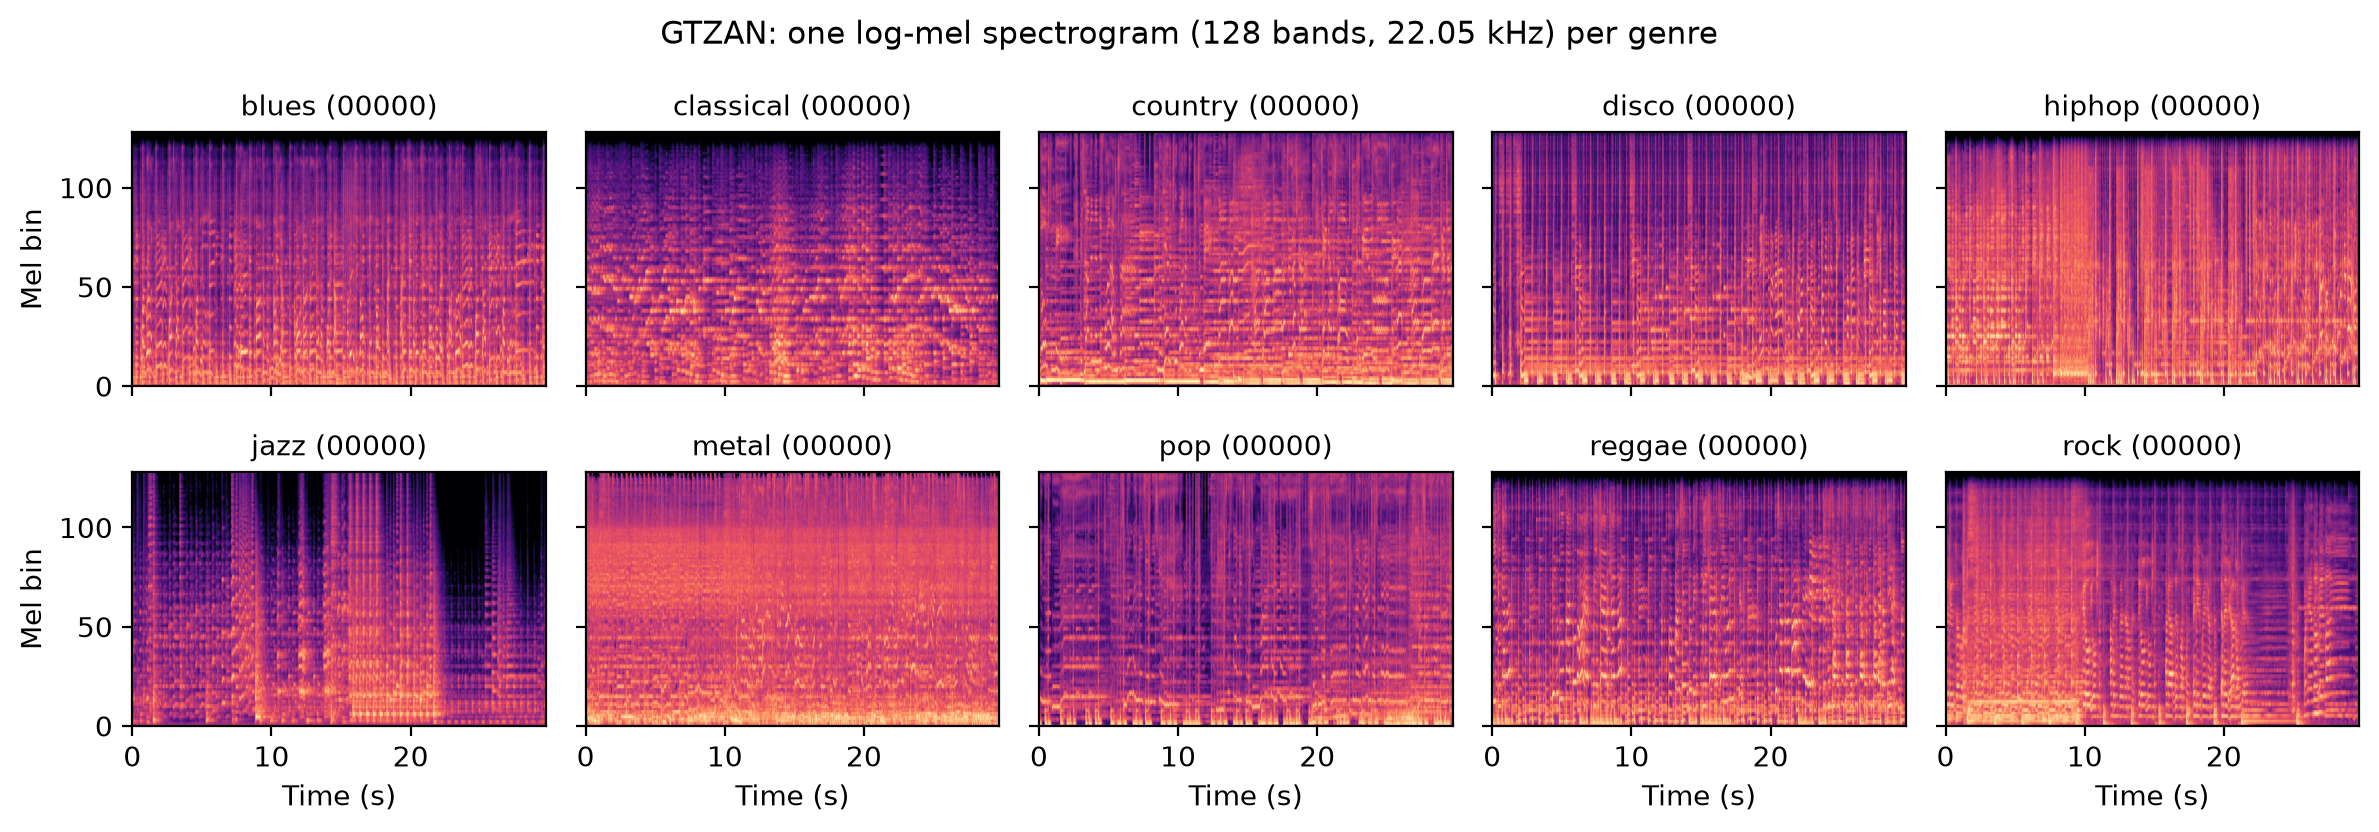
\includegraphics[width=0.94\textwidth]{dataset_samples.png}
\caption{Sample data: the log-mel spectrogram (128 bands, first 29.7\,s) of the first clip of each GTZAN genre.}
\label{fig:samples}
\end{figure*}

\textbf{Spotify tracks.} For mood we use a public dataset of 114{,}000 tracks collected through the Spotify Web API\footnote{\url{https://huggingface.co/datasets/maharshipandya/spotify-tracks-dataset}}. Removing duplicate track IDs leaves 89{,}741 tracks with 113 genre labels. Each track carries Spotify's audio descriptors; we use danceability, loudness, tempo, acousticness, instrumentalness, speechiness, liveness, mode and key as inputs. The quadrant labels are unbalanced: 33{,}221 \emph{happy} (37.0\%), 30{,}211 \emph{tense} (33.7\%), 19{,}030 \emph{sad} (21.2\%) and only 7{,}279 \emph{calm} (8.1\%). Table~\ref{tab:spotify} lists one popular track from each class.

\begin{table}[t]
\caption{Sample Spotify tracks (one per mood quadrant)}
\label{tab:spotify}
\centering
\setlength{\tabcolsep}{3.5pt}
\begin{tabular}{@{}lrrrrl@{}}
\toprule
Track (artist) & Val. & Energy & Dance. & Loud. & Mood\\
\midrule
Bzrp Music Sessions 52 (Bizarrap) & 0.55 & 0.78 & 0.62 & $-5.5$ & happy\\
I'm Good (Blue) (D.\ Guetta) & 0.30 & 0.97 & 0.56 & $-3.7$ & tense\\
Unholy (Sam Smith) & 0.24 & 0.47 & 0.71 & $-7.4$ & sad\\
c\'omo dormiste? (Rels B) & 0.57 & 0.43 & 0.63 & $-8.3$ & calm\\
\bottomrule
\end{tabular}
\end{table}

\section{Methodology}
Fig.~\ref{fig:pipeline} summarises the three pipelines.

\begin{figure*}[t]
\centering
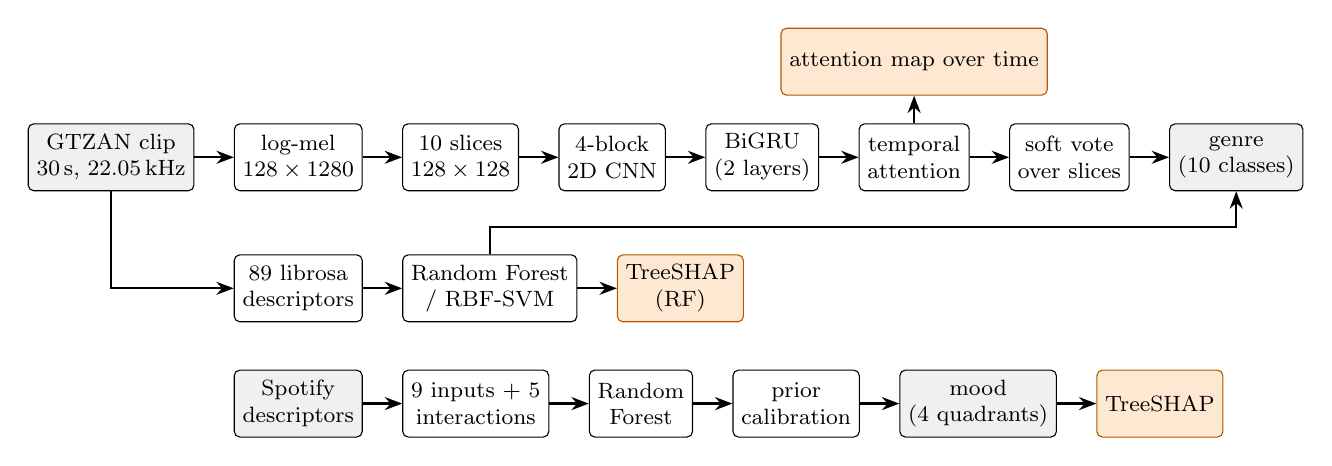
\begin{tikzpicture}[
  font=\footnotesize,
  box/.style={draw, rounded corners=2pt, align=center, minimum height=8.5mm, inner sep=3pt, fill=white},
  data/.style={box, fill=gray!12},
  expl/.style={box, fill=orange!18, draw=orange!70!black},
  arr/.style={-{Stealth[length=2.2mm]}, thick},
  node distance=4.5mm and 5mm]
% genre, deep branch
\node[data] (audio) {GTZAN clip\\30\,s, 22.05\,kHz};
\node[box, right=of audio] (mel) {log-mel\\$128\times1280$};
\node[box, right=of mel] (slice) {10 slices\\$128\times128$};
\node[box, right=of slice] (cnn) {4-block\\2D CNN};
\node[box, right=of cnn] (gru) {BiGRU\\(2 layers)};
\node[box, right=of gru] (att) {temporal\\attention};
\node[box, right=of att] (vote) {soft vote\\over slices};
\node[data, right=of vote] (genre) {genre\\(10 classes)};
\node[expl, above=3.5mm of att] (attx) {attention map over time};
% genre, classical branch
\node[box, below=8mm of mel] (feat) {89 librosa\\descriptors};
\node[box, right=of feat] (rf) {Random Forest\\/ RBF-SVM};
\node[expl, right=of rf] (shapg) {TreeSHAP\\(RF)};
% mood branch
\node[data, below=6mm of feat] (spot) {Spotify\\descriptors};
\node[box, right=of spot] (inter) {9 inputs + 5\\interactions};
\node[box, right=of inter] (mrf) {Random\\Forest};
\node[box, right=of mrf] (cal) {prior\\calibration};
\node[data, right=of cal] (mood) {mood\\(4 quadrants)};
\node[expl, right=of mood] (shapm) {TreeSHAP};
\draw[arr] (audio) -- (mel); \draw[arr] (mel) -- (slice); \draw[arr] (slice) -- (cnn);
\draw[arr] (cnn) -- (gru); \draw[arr] (gru) -- (att); \draw[arr] (att) -- (vote); \draw[arr] (vote) -- (genre);
\draw[arr] (att) -- (attx);
\draw[arr] (audio.south) |- (feat.west); \draw[arr] (feat) -- (rf); \draw[arr] (rf) -- (shapg);
\draw[arr] (rf.north) -- ++(0,3.5mm) -| (genre.south);
\draw[arr] (spot) -- (inter); \draw[arr] (inter) -- (mrf); \draw[arr] (mrf) -- (cal); \draw[arr] (cal) -- (mood); \draw[arr] (mood) -- (shapm);
\end{tikzpicture}
\caption{Methodology. Top: Attention-CRNN on 3\,s slices with song-level soft voting. Middle: handcrafted-feature baselines. Bottom: mood classification on Spotify descriptors. Orange boxes are the explanations we produce.}
\label{fig:pipeline}
\end{figure*}

\subsection{Handcrafted features and classical baselines}
For each clip we compute, with librosa 0.11, 20 MFCCs, 12 chroma bins, spectral centroid, bandwidth and roll-off, 7-band spectral contrast, zero-crossing rate and RMS energy, and keep the mean and standard deviation of each over time. Adding a global tempo estimate gives 89 named features. Tempo comes from the autocorrelation of the onset-strength envelope restricted to 40--240\,BPM; we use this instead of librosa's beat tracker, which crashed on our Apple Silicon machines. The baselines are a Random Forest with 300 trees and an SVM with an RBF kernel ($C=10$) on standardised features.

\subsection{Attention-CNN on full clips}
Our first network reads the whole $128\times1280$ spectrogram. Four convolution blocks (32, 64, 128 and 256 filters of size $3\times3$, each with batch normalisation, ReLU and max pooling) are followed by adaptive pooling to 40 time steps of 256 features. A small attention layer (256$\to$64$\to$1 with tanh) weights the 40 steps, and the weighted sum feeds a dropout (0.4) and linear classifier. The model has 407{,}883 parameters.

\subsection{Attention-CRNN on 3\,s slices}
The CRNN applies the same idea at a finer scale. Each $128\times128$ slice passes through four convolution blocks with pooling sizes $(2,2)$, $(2,2)$, $(4,2)$ and $(8,1)$, which collapse the frequency axis and leave 16 time steps of 256 features. A two-layer bidirectional GRU (128 units per direction, dropout 0.25) models their order, and the attention of~\eqref{eq:attn} pools them. A dropout of 0.35 and a linear layer give the slice logits, and~\eqref{eq:vote} combines the ten slices. The model has 1{,}017{,}290 parameters. Slicing multiplies the number of training examples by ten, and the vote lets confident slices outweigh ambiguous ones.

To avoid leakage, we split GTZAN by song (stratified 80/20, seed 42) \emph{before} slicing, so no slice of a test song is ever seen in training. Both networks and both classical baselines are evaluated on the same 200 test songs.

\subsection{Mood classifier}
The mood model is a Random Forest on the nine Spotify inputs plus five interaction features meant to capture combinations that separate the quadrants: loudness$\times$danceability, acousticness$\times$instrumentalness, acousticness$/(|\text{loudness}|+1)$, danceability$\times$tempo and speechiness$/(\text{acousticness}+0.01)$. Because \emph{calm} covers only 8\% of tracks, the forest rarely predicts it; multiplying its probability by 1.45 before the argmax trades a little precision on the other classes for calm recall.

\subsection{Explanations and demonstration}
We compute TreeSHAP values for the genre Random Forest and the mood forest, both per song and averaged over the test set. For the CRNN we keep the attention weights of all ten slices, which gives 160 weights over the clip. A separate script places local SHAP values next to the CRNN attention curve for the same test songs.

All models are also packaged in a web application with a FastAPI back end and a React front end. A user can upload a song, play it while the attention curve scrolls under the spectrogram, see each slice's vote and compare the four models. The code is available on GitHub\footnote{\url{https://github.com/devanshrai23/iml-music-genre-mood}} and a public version of the site is deployed\footnote{\url{https://iml-music-genre-mood.vercel.app/}}.

\section{Experimental Settings}
Table~\ref{tab:settings} lists the training settings. Both networks use AdamW~\cite{loshchilov2019} with a cosine learning-rate schedule and SpecAugment-style masking~\cite{park2019} on the training data. All experiments ran on a MacBook Air (Apple M5) using the PyTorch MPS back end (PyTorch 2.14, scikit-learn 1.9, shap 0.51, Python 3.11). Each training script logs the loss and accuracy of every epoch so that the curves in Fig.~\ref{fig:loss} can be regenerated from the repository.

\begin{table}[t]
\caption{Training settings}
\label{tab:settings}
\centering
\setlength{\tabcolsep}{4pt}
\begin{tabular}{@{}lll@{}}
\toprule
 & Attention-CNN & Attention-CRNN\\
\midrule
Input & $128\times1280$ clip & $128\times128$ slice\\
Training examples & 799 clips & 7{,}990 slices\\
Batch size / epochs & 32 / 25 & 64 / 30\\
Learning rate, weight decay & $10^{-3}$, $10^{-2}$ & $10^{-3}$, $10^{-4}$\\
Loss & cross-entropy & CE, label smoothing 0.05\\
Masking (per example) & 1 time (20--80 fr.), & 1 time, 1 freq.\\
 & 1 freq.\ (5--16 bins) & (0--16 each)\\
Dropout & 0.4 & 0.25 (GRU), 0.35\\
Parameters & 407{,}883 & 1{,}017{,}290\\
\bottomrule
\end{tabular}
\end{table}

\textbf{Evaluation protocols.} The Random Forest and SVM are reported with stratified 5-fold cross-validation on all 999 clips and on the 200-song test split used for the networks. The networks are trained once with seed 42; we keep the epoch with the best song-level test accuracy, a choice we return to in Section~\ref{sec:conclusion}. The mood models are evaluated with stratified 5-fold cross-validation on all 89{,}741 tracks; the per-class figures in Table~\ref{tab:mood} come from an 80/20 hold-out split. We report accuracy and macro-averaged precision, recall and F1, since the mood classes are unbalanced.

\section{Results and Analysis}

\subsection{Genre classification}
Table~\ref{tab:main} gives the main results. The networks beat the feature-based models by a clear margin, and the CRNN is best at 87.0\% accuracy and 0.869 macro-F1. The Random Forest drops from 74.5\% under cross-validation to 72.0\% on the fixed split, while the SVM rises from 77.6\% to 80.5\%; with 200 test songs each song is worth 0.5 points, so the gap between protocols is within the noise of a single split.

\begin{table}[t]
\caption{Genre results on GTZAN (accuracy and macro-F1)}
\label{tab:main}
\centering
\setlength{\tabcolsep}{4pt}
\begin{tabular}{@{}lcccc@{}}
\toprule
 & \multicolumn{2}{c}{5-fold CV (999)} & \multicolumn{2}{c}{Test split (200)}\\
Model & Acc. & F1 & Acc. & F1\\
\midrule
Random Forest (89 features) & 74.5 & 0.740 & 72.0 & 0.717\\
RBF-SVM (89 features) & 77.6 & 0.776 & 80.5 & 0.802\\
Attention-CNN (30\,s clip) & -- & -- & 83.0 & 0.827\\
Attention-CRNN (10$\times$3\,s, vote) & -- & -- & \textbf{87.0} & \textbf{0.869}\\
\bottomrule
\end{tabular}
\end{table}

Table~\ref{tab:pergenre} breaks the test-split F1 down by genre. Classical, metal and jazz are almost solved by the CRNN. The largest improvements over the Random Forest are on rock (0.47 to 0.74), blues (0.67 to 0.92) and reggae (0.58 to 0.81). Rock remains the hardest class: the CRNN labels 3 of the 20 rock songs as pop and 2 as hip-hop (Fig.~\ref{fig:cm}). Pop is the one genre where the CRNN is clearly worse than the CNN (0.76 against 0.85), partly because three rock songs are predicted as pop.

\begin{table}[t]
\caption{Per-genre F1 on the 200-song test split}
\label{tab:pergenre}
\centering
\begin{tabular}{@{}lcccc@{}}
\toprule
Genre & RF & SVM & CNN & CRNN\\
\midrule
Blues & 0.67 & 0.85 & 0.82 & \textbf{0.92}\\
Classical & 0.92 & 0.95 & \textbf{0.98} & \textbf{0.98}\\
Country & 0.70 & 0.80 & 0.74 & \textbf{0.88}\\
Disco & 0.58 & 0.69 & \textbf{0.82} & 0.81\\
Hip-hop & 0.70 & 0.77 & \textbf{0.88} & 0.86\\
Jazz & 0.86 & 0.91 & 0.88 & \textbf{0.95}\\
Metal & 0.88 & 0.87 & 0.86 & \textbf{0.97}\\
Pop & 0.81 & 0.79 & \textbf{0.85} & 0.76\\
Reggae & 0.58 & 0.67 & \textbf{0.86} & 0.81\\
Rock & 0.47 & 0.72 & 0.57 & \textbf{0.74}\\
\midrule
Macro average & 0.717 & 0.802 & 0.827 & \textbf{0.869}\\
\bottomrule
\end{tabular}
\end{table}

\begin{figure}[t]
\centering
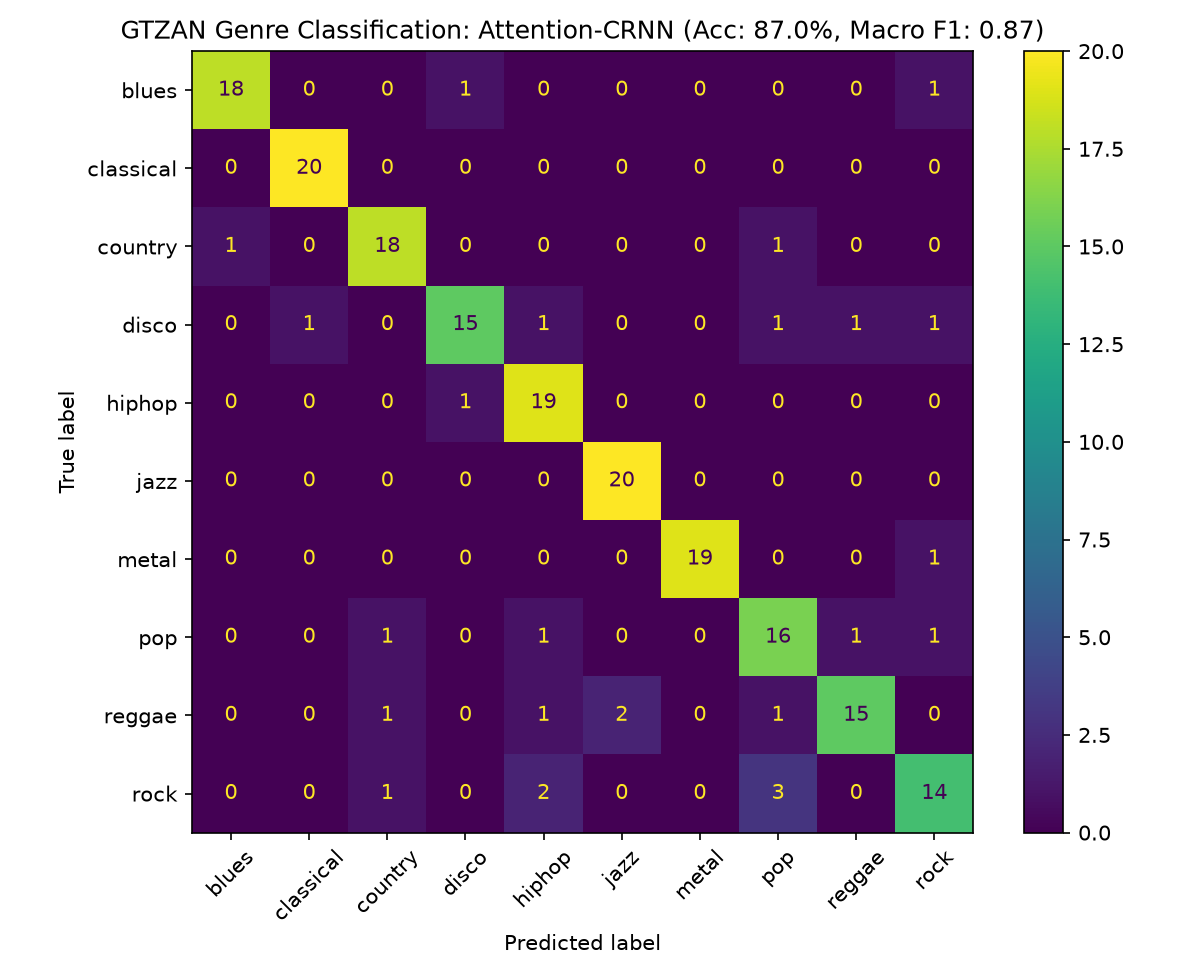
\includegraphics[width=0.92\columnwidth]{confusion_CRNN.png}
\caption{Confusion matrix of the Attention-CRNN on the 200 test songs (rows: true genre).}
\label{fig:cm}
\end{figure}

\subsection{Training behaviour}
Fig.~\ref{fig:loss} plots the loss and accuracy of both networks for every epoch. The CRNN's training loss falls from 1.46 to 0.31; it cannot reach zero because of label smoothing. Its slice-level test loss stops improving after about ten epochs and settles near 0.70, while the training loss keeps falling, so the model overfits mildly in the second half of training. The CNN trains much less smoothly. Its test accuracy collapses to 19.5\% at epoch 4 and 49.5\% at epoch 13 before recovering. The CRNN drops sharply only once, to 40\% at epoch 2, and stays at or above 74\% from epoch 3 onwards. We attribute the difference to batch size and data volume: the CNN sees 799 long clips in batches of 32, so its batch-normalisation statistics and gradients vary more between steps than those of the CRNN, which sees 7{,}990 slices in batches of 64.

\begin{figure*}[t]
\centering
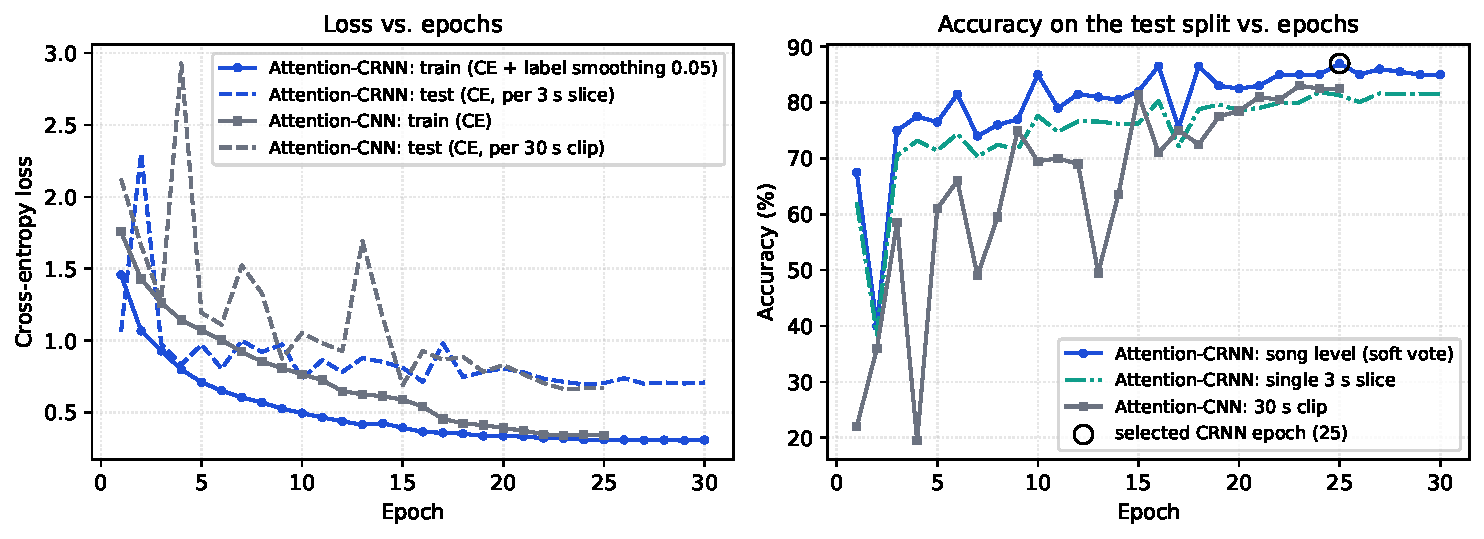
\includegraphics[width=0.9\textwidth]{training_loss_curve.pdf}
\caption{Training loss vs.\ epochs (left) and test accuracy vs.\ epochs (right) for the Attention-CNN and Attention-CRNN, drawn from the per-epoch logs. The CRNN training loss includes label smoothing; evaluation losses are plain cross-entropy. The circle marks the CRNN epoch kept for testing.}
\label{fig:loss}
\end{figure*}

\subsection{Ablation study}
Table~\ref{tab:ablation} removes one CRNN component at a time and retrains with the same seed and schedule. The clearest effect comes from slicing and voting. A single 3\,s slice is classified correctly 81.3\% of the time; averaging ten of them raises song accuracy to 87.0\%, and the CRNN beats the full-clip CNN by four points. The other components matter much less. Replacing attention with uniform weights (mean pooling) costs 0.5 points, removing SpecAugment costs 1.0 point, and replacing the GRU by a per-step linear layer leaves accuracy unchanged at 87.0\% with half the parameters. These differences correspond to one or two songs. A 95\% binomial confidence interval for 87\% accuracy on 200 songs is roughly $\pm4.7$ points, so we cannot claim that attention, the GRU or SpecAugment improve accuracy on GTZAN. What we can say is that attention costs nothing in accuracy and gives us the time-level explanation.

\begin{table}[t]
\caption{CRNN ablations on the 200-song test split}
\label{tab:ablation}
\centering
\setlength{\tabcolsep}{3.5pt}
\begin{tabular}{@{}lcccc@{}}
\toprule
Configuration & Params & Song acc. & Slice acc. & F1\\
\midrule
Full Attention-CRNN & 1.02\,M & 87.0 & 81.3 & 0.869\\
w/o attention (mean pool) & 0.98\,M & 86.5 & 80.0 & 0.867\\
w/o BiGRU (linear per step) & 0.49\,M & 87.0 & 81.0 & 0.870\\
w/o SpecAugment & 1.02\,M & 86.0 & 81.3 & 0.862\\
w/o slicing (Attention-CNN) & 0.41\,M & 83.0 & -- & 0.827\\
\bottomrule
\end{tabular}
\end{table}

\subsection{Mood classification}
Table~\ref{tab:mood} shows the mood results. The baseline forest on the nine raw inputs reaches 70.5\% accuracy but only 0.660 macro-F1, because it rarely predicts \emph{calm}. Adding interaction features and the 1.45 prior boost lowers accuracy slightly to 70.1\% and raises macro-F1 to 0.667. On the hold-out split the boost lifts calm recall from 0.33 to 0.47 (0.36 to 0.48 under cross-validation); the main cost is sad recall, which falls from 0.80 to 0.77. Calm remains the weakest class (F1 0.49), which is expected: it is the smallest class, and without valence the model has to separate a quiet happy song from a quiet sad one using danceability, loudness and acousticness alone. Danceability and loudness have the largest mean |SHAP| values for \emph{happy}, and loudness is the strongest feature for \emph{calm}.

\begin{table}[t]
\caption{Mood results (Spotify, 4 classes)}
\label{tab:mood}
\centering
\setlength{\tabcolsep}{4pt}
\begin{tabular}{@{}llccc@{}}
\toprule
Model & Protocol & Acc. & F1 & Calm rec.\\
\midrule
RF, 9 inputs & 5-fold CV & 70.5 & 0.660 & --\\
RF + interactions + prior & 5-fold CV & 70.1 & 0.667 & 0.48\\
RF + interactions, no prior & 80/20 split & 69.6 & 0.646 & 0.33\\
RF + interactions + prior & 80/20 split & 69.6 & 0.663 & 0.47\\
\bottomrule
\end{tabular}
\end{table}

\subsection{What the explanations show}
Averaged over the test songs, the most important features for the genre forest are the mean spectral contrast in bands 5 and 4, the standard deviation of MFCC~5, mean RMS energy and the variability of the spectral centroid. These describe how peaky the spectrum is in the upper-middle range and how loud and how changeable the clip is, which fits the classes the forest separates well (classical and metal) and those it confuses (rock, disco and reggae, which share band-limited, compressed mixes).

Fig.~\ref{fig:shapatt} compares the two explanations on two test songs. For a classical clip that both models get right, SHAP credits low RMS energy and the first MFCC (overall loudness and spectral tilt), and the CRNN is 96\% confident. For a disco clip the forest calls hip-hop, the largest SHAP contributions come from spectral contrast in bands 4 and 5, so the forest is reacting to the dense, compressed spectrum that disco shares with hip-hop. The CRNN labels it correctly, with 50\% confidence. One property of~\eqref{eq:attn} needs care when reading these plots: the softmax runs separately inside each slice, so every slice produces a peak by construction. Peak heights can be compared within a slice but not between slices, and the curve says where the model looked, not that the region it looked at is ``disco''. This is the concern raised by Jain and Wallace~\cite{jain2019}, and our ablation adds a practical point: on this data, uniform weights work almost as well as learned ones.

\begin{figure}[t]
\centering
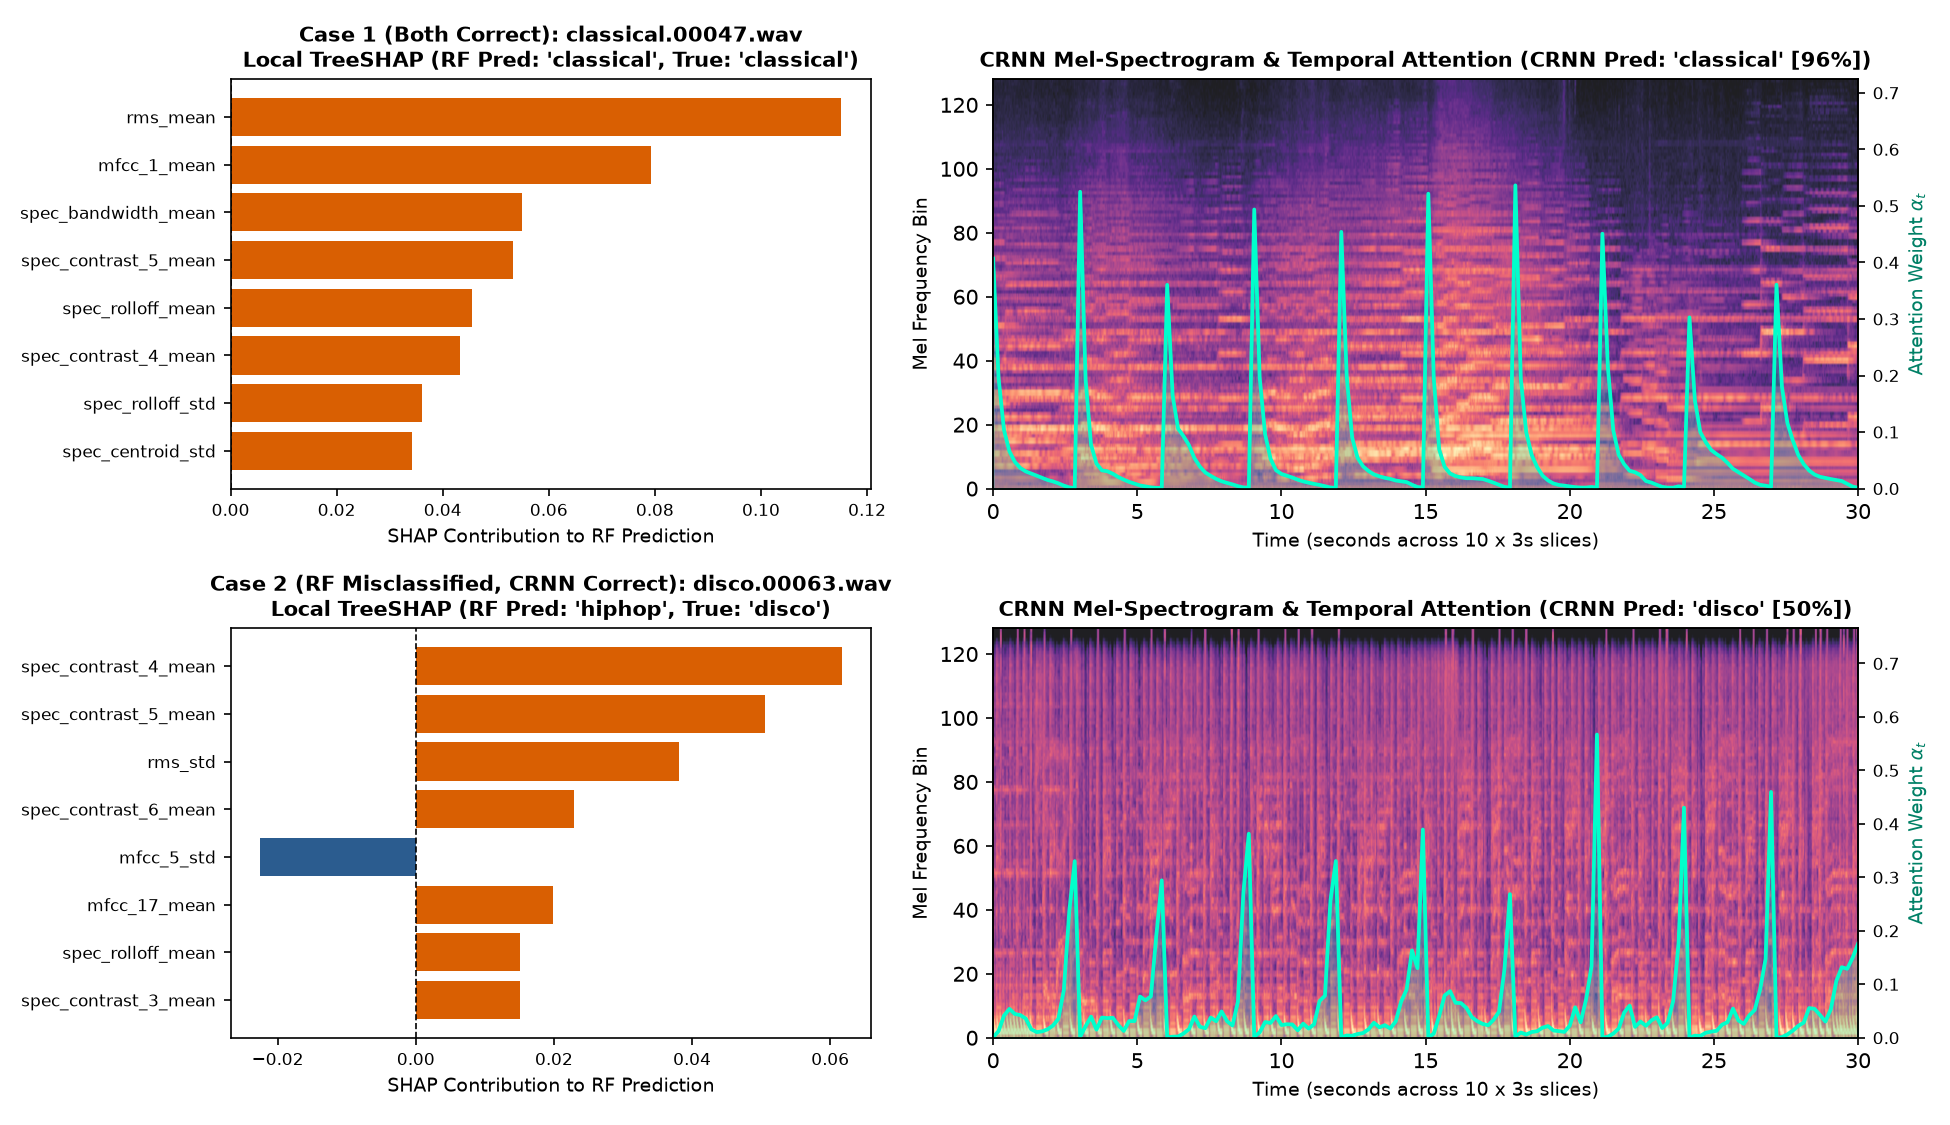
\includegraphics[width=\columnwidth]{shap_vs_attention_comparison.png}
\caption{Local TreeSHAP values of the Random Forest (left) and CRNN attention over the spectrogram (right) for a classical song both models classify correctly (top) and a disco song the forest misclassifies as hip-hop (bottom).}
\label{fig:shapatt}
\end{figure}

\section{Conclusion}
\label{sec:conclusion}
On GTZAN, an Attention-CRNN that votes over ten 3\,s slices reached 87.0\% accuracy on 200 held-out songs, against 72.0\% for a Random Forest on handcrafted features. The ablations point to slicing and soft voting as the source of most of this gain; attention, recurrence and SpecAugment change accuracy by at most one point. For mood, a calibrated Random Forest reached 0.667 macro-F1 on 89{,}741 Spotify tracks without access to the valence and energy fields that define the labels.

The results have limits that we want to state plainly. First, we chose the networks' best epoch using test-set accuracy, so 87.0\% is an optimistic estimate; our training scripts now support a separate validation split (\texttt{--val-frac}) to remove this bias. Second, all networks were trained with a single seed, and a 200-song test set gives a confidence interval of about $\pm4.7$ points, which is wider than every difference in Table~\ref{tab:ablation}. Third, GTZAN is small, dated and known to be problematic as a benchmark~\cite{sturm2014}, so our accuracy says little about performance on current music. Fourth, the mood model depends on Spotify's precomputed descriptors and cannot label a new audio file.

The web demo has related limits. The models only know ten genres, so a song outside them (for example a Bollywood track) is forced into the closest one. The public deployment on Vercel cannot run PyTorch, so it shows 20 precomputed test songs without audio playback; uploading new audio and moving the mood sliders work only when the Python back end is running locally. Future work includes validation-based model selection with several seeds, training on a larger dataset such as the Free Music Archive, a mood model that works from raw audio, and hosting the back end so that uploads work online.

%% Optional, if your course requires disclosure of tool use:
%\section*{Acknowledgment}
%Parts of the code and an early draft of this report were prepared with the help of an AI assistant; all experiments were run and all text was checked by the authors.

\begin{thebibliography}{00}
\bibitem{tzanetakis2002} G. Tzanetakis and P. Cook, ``Musical genre classification of audio signals,'' \textit{IEEE Trans. Speech Audio Process.}, vol.~10, no.~5, pp.~293--302, Jul. 2002.
\bibitem{russell1980} J. A. Russell, ``A circumplex model of affect,'' \textit{J. Pers. Soc. Psychol.}, vol.~39, no.~6, pp.~1161--1178, 1980.
\bibitem{sturm2014} B. L. Sturm, ``The state of the art ten years after a state of the art: Future research in music information retrieval,'' \textit{J. New Music Res.}, vol.~43, no.~2, pp.~147--172, 2014.
\bibitem{choi2017} K. Choi, G. Fazekas, M. Sandler, and K. Cho, ``Convolutional recurrent neural networks for music classification,'' in \textit{Proc. IEEE Int. Conf. Acoust., Speech Signal Process. (ICASSP)}, 2017, pp.~2392--2396.
\bibitem{prabhakar2023} S. K. Prabhakar and S.-W. Lee, ``Holistic approaches to music genre classification using efficient transfer and deep learning techniques,'' \textit{Expert Syst. Appl.}, vol.~211, Art.~no.~118636, 2023.
\bibitem{park2019} D. S. Park, W. Chan, Y. Zhang, C.-C. Chiu, B. Zoph, E. D. Cubuk, and Q. V. Le, ``SpecAugment: A simple data augmentation method for automatic speech recognition,'' in \textit{Proc. Interspeech}, 2019, pp.~2613--2617.
\bibitem{panda2023} R. Panda, R. Malheiro, and R. P. Paiva, ``Audio features for music emotion recognition: A survey,'' \textit{IEEE Trans. Affect. Comput.}, vol.~14, no.~1, pp.~68--88, 2023.
\bibitem{lundberg2017} S. M. Lundberg and S.-I. Lee, ``A unified approach to interpreting model predictions,'' in \textit{Adv. Neural Inf. Process. Syst. (NeurIPS)}, vol.~30, 2017, pp.~4765--4774.
\bibitem{lundberg2020} S. M. Lundberg, G. Erion, H. Chen, A. DeGrave, J. M. Prutkin, B. Nair, R. Katz, J. Himmelfarb, N. Bansal, and S.-I. Lee, ``From local explanations to global understanding with explainable AI for trees,'' \textit{Nature Mach. Intell.}, vol.~2, no.~1, pp.~56--67, 2020.
\bibitem{jain2019} S. Jain and B. C. Wallace, ``Attention is not explanation,'' in \textit{Proc. NAACL-HLT}, 2019, pp.~3543--3556.
\bibitem{wiegreffe2019} S. Wiegreffe and Y. Pinter, ``Attention is not not explanation,'' in \textit{Proc. EMNLP-IJCNLP}, 2019, pp.~11--20.
\bibitem{loshchilov2019} I. Loshchilov and F. Hutter, ``Decoupled weight decay regularization,'' in \textit{Proc. Int. Conf. Learn. Represent. (ICLR)}, 2019.
\end{thebibliography}

\end{document}
